% 21_inferencia.tex: de la población a la muestra y vuelta (descriptiva vs inferencial)
% (standalone; TikZ choca con ctable en la presentación) -> img/inferencia.pdf
\documentclass[border=3pt]{standalone}
\usepackage[utf8]{inputenc}
\usepackage{mathpazo}
\usepackage{tikz}
\usetikzlibrary{positioning,fit,backgrounds,arrows.meta}
\begin{document}
\footnotesize
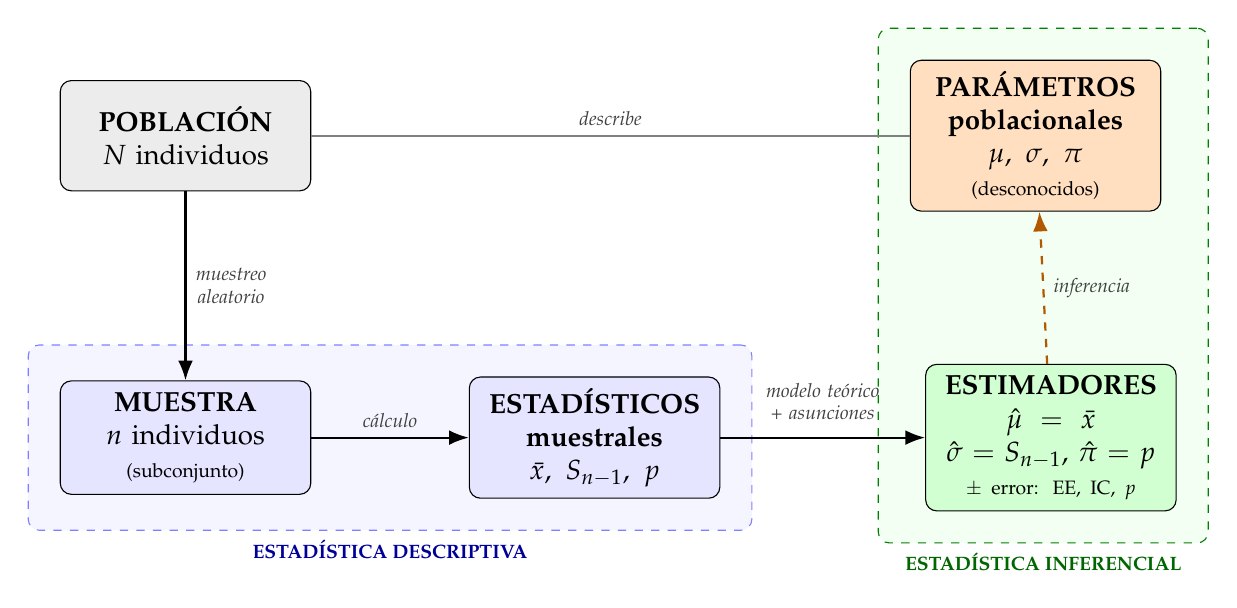
\begin{tikzpicture}[
  node distance=14mm and 16mm,
  caja/.style={draw, rounded corners, align=center, inner sep=4pt, minimum height=14mm, text width=29mm},
  pob/.style={caja, fill=gray!15},
  par/.style={caja, fill=orange!25},
  mue/.style={caja, fill=blue!10},
  est/.style={caja, fill=blue!10},
  inf/.style={caja, fill=green!18},
  flecha/.style={-{Latex[length=2.5mm]}, thick},
  rotulo/.style={font=\scriptsize\itshape, align=center, text=black!75}]

% --- fila superior: la realidad (inobservable)
\node[pob] (pob) {\textbf{POBLACIÓN}\\ $N$ individuos};
\node[par, right=76mm of pob] (par) {\textbf{PARÁMETROS}\\ \textbf{poblacionales}\\ $\mu,\ \sigma,\ \pi$ \\ {\scriptsize (desconocidos)}};

% --- fila inferior: lo que observamos
\node[mue, below=24mm of pob] (mue) {\textbf{MUESTRA}\\ $n$ individuos\\ {\scriptsize (subconjunto)}};
\node[est, right=20mm of mue] (est) {\textbf{ESTADÍSTICOS}\\ \textbf{muestrales}\\ $\bar{x},\ S_{n-1},\ p$};
\node[inf, right=26mm of est] (inf) {\textbf{ESTIMADORES}\\ $\hat\mu=\bar{x}$\\ $\hat\sigma=S_{n-1}$,\ $\hat\pi=p$\\ {\scriptsize $\pm$ error: EE, IC, $p$}};

% --- flechas
\draw[flecha] (pob) -- node[rotulo, right] {muestreo\\aleatorio} (mue);
\draw[flecha] (mue) -- node[rotulo, above] {cálculo} (est);
\draw[flecha] (est) -- node[rotulo, above=1mm, text width=26mm] {modelo teórico\\+ asunciones} (inf);
\draw[flecha, dashed, orange!70!black] (inf) -- node[rotulo, right] {inferencia} (par);
\draw[thick, gray] (pob) -- node[rotulo, above] {describe} (par);

% --- bandas
\begin{scope}[on background layer]
 \node[draw=blue!50, dashed, rounded corners, fill=blue!4, fit=(mue)(est), inner sep=4mm,
   label={[blue!60!black, font=\scriptsize\bfseries]below:ESTADÍSTICA DESCRIPTIVA}] {};
 \node[draw=green!50!black, dashed, rounded corners, fill=green!5, fit=(inf)(par), inner sep=4mm,
   label={[green!40!black, font=\scriptsize\bfseries]below:ESTADÍSTICA INFERENCIAL}] {};
\end{scope}
\end{tikzpicture}
\end{document}
